% Exercise 2.3

\begin{itemize}
    \item[(a)] We have the following R plot of various error curves:
    \begin{figure}[!ht]
        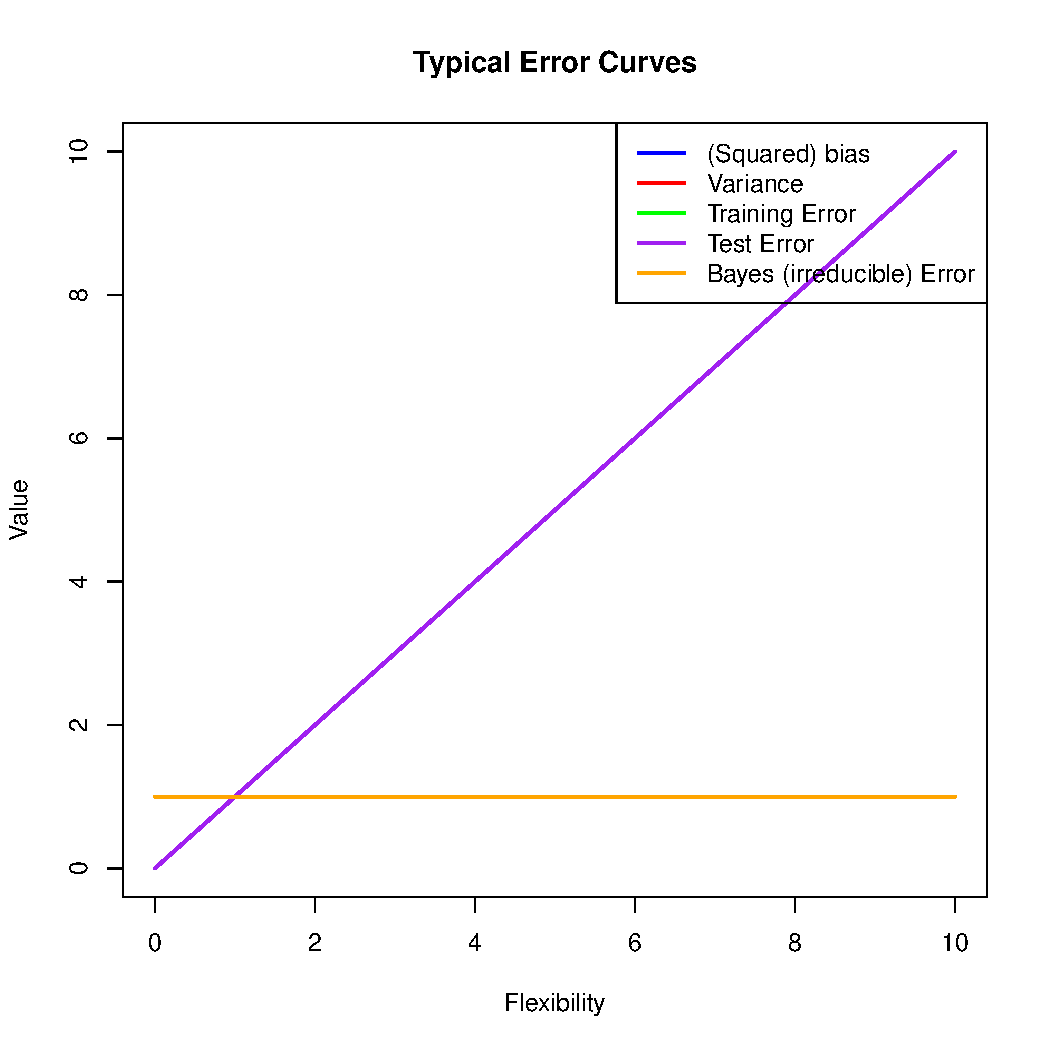
\includegraphics[scale=0.6, center]{../plots/ex2_3_a.pdf}
        \caption{
            Typical (squared) bias, variance, training error, test error, and Bayes 
            (irreducible) error
        }\label{fig:figure1}
    \end{figure}
    Arbitrary polynomials of the appropriate degree were used to generate these 
    plots, since they are approximations, using the following script:
    \begin{verbatim}
# Exercise 2.3(a) - Plots of error curves

squared_bias <- function(x) {
  return((x - 1.25)^4 + 0.01 * x^3 + 0.05 * x^2 - 0.1 * x + 1.15)
}

variance <- function(x) {
  return((x - 1.25)^4 + 0.01 * x^3 + 0.05 * x^2 - 0.1 * x + 0.25)
}

training_err <- function(x) {
  return((x - 1.25)^4 + 0.01 * x^3 + 0.05 * x^2 - 0.1 * x + 1.25)
}

test_err <- function(x) {
  return(-(x - 1.25)^3 + 0.05 * x^2 - 0.1 * x + 1.0)
}

bayes_err <- function(x) {
  return(rep(1.0, length(x)))
}

x <- seq(0, 2.5, by = 0.1)

y1 <- squared_bias(x)
y2 <- variance(x)
y3 <- training_err(x)
y4 <- test_err(x)
y5 <- bayes_err(x)

pdf("ex2_3_a.pdf")

plot(x, y1,
  type = "l", col = "blue", lwd = 1, ylim = c(0, 2.5), xlab = "Flexibility",
  ylab = "Value", main = "Typical Error Curves"
)

lines(x, y2, col = "red", lwd = 1)
lines(x, y3, col = "green", lwd = 1)
lines(x, y4, col = "orange", lwd = 1)
lines(x, y5, col = "gray", lwd = 1, lty = 2)

legend("topright",
  legend = c(
    "(Squared) bias", "Variance", "Training Error", "Test Error",
    "Bayes (irreducible) Error"
  ),
  col = c("blue", "red", "green", "orange", "gray"), lwd = 1
)

dev.off()

    \end{verbatim}
  \item[(b)] We are given that the training error will always be greater than
  the (squared) bias, and that both will be u-shaped. The variance will always
  be less than the (squared) bias, while the test error will decrease as the model
  becomes more flexible. The Bayes error is irreducible, so it remains constant.
\end{itemize}
